\documentclass[twoside]{book}

% Packages required by doxygen
\usepackage{fixltx2e}
\usepackage{calc}
\usepackage{doxygen}
\usepackage[export]{adjustbox} % also loads graphicx
\usepackage{graphicx}
\usepackage[utf8]{inputenc}
\usepackage{makeidx}
\usepackage{multicol}
\usepackage{multirow}
\PassOptionsToPackage{warn}{textcomp}
\usepackage{textcomp}
\usepackage[nointegrals]{wasysym}
\usepackage[table]{xcolor}

% Font selection
\usepackage[T1]{fontenc}
\usepackage[scaled=.90]{helvet}
\usepackage{courier}
\usepackage{amssymb}
\usepackage{sectsty}
\renewcommand{\familydefault}{\sfdefault}
\allsectionsfont{%
  \fontseries{bc}\selectfont%
  \color{darkgray}%
}
\renewcommand{\DoxyLabelFont}{%
  \fontseries{bc}\selectfont%
  \color{darkgray}%
}
\newcommand{\+}{\discretionary{\mbox{\scriptsize$\hookleftarrow$}}{}{}}

% Page & text layout
\usepackage{geometry}
\geometry{%
  a4paper,%
  top=2.5cm,%
  bottom=2.5cm,%
  left=2.5cm,%
  right=2.5cm%
}
\tolerance=750
\hfuzz=15pt
\hbadness=750
\setlength{\emergencystretch}{15pt}
\setlength{\parindent}{0cm}
\setlength{\parskip}{3ex plus 2ex minus 2ex}
\makeatletter
\renewcommand{\paragraph}{%
  \@startsection{paragraph}{4}{0ex}{-1.0ex}{1.0ex}{%
    \normalfont\normalsize\bfseries\SS@parafont%
  }%
}
\renewcommand{\subparagraph}{%
  \@startsection{subparagraph}{5}{0ex}{-1.0ex}{1.0ex}{%
    \normalfont\normalsize\bfseries\SS@subparafont%
  }%
}
\makeatother

% Headers & footers
\usepackage{fancyhdr}
\pagestyle{fancyplain}
\fancyhead[LE]{\fancyplain{}{\bfseries\thepage}}
\fancyhead[CE]{\fancyplain{}{}}
\fancyhead[RE]{\fancyplain{}{\bfseries\leftmark}}
\fancyhead[LO]{\fancyplain{}{\bfseries\rightmark}}
\fancyhead[CO]{\fancyplain{}{}}
\fancyhead[RO]{\fancyplain{}{\bfseries\thepage}}
\fancyfoot[LE]{\fancyplain{}{}}
\fancyfoot[CE]{\fancyplain{}{}}
\fancyfoot[RE]{\fancyplain{}{\bfseries\scriptsize Generated by Doxygen }}
\fancyfoot[LO]{\fancyplain{}{\bfseries\scriptsize Generated by Doxygen }}
\fancyfoot[CO]{\fancyplain{}{}}
\fancyfoot[RO]{\fancyplain{}{}}
\renewcommand{\footrulewidth}{0.4pt}
\renewcommand{\chaptermark}[1]{%
  \markboth{#1}{}%
}
\renewcommand{\sectionmark}[1]{%
  \markright{\thesection\ #1}%
}

% Indices & bibliography
\usepackage{natbib}
\usepackage[titles]{tocloft}
\setcounter{tocdepth}{3}
\setcounter{secnumdepth}{5}
\makeindex

% Hyperlinks (required, but should be loaded last)
\usepackage{ifpdf}
\ifpdf
  \usepackage[pdftex,pagebackref=true]{hyperref}
\else
  \usepackage[ps2pdf,pagebackref=true]{hyperref}
\fi
\hypersetup{%
  colorlinks=true,%
  linkcolor=blue,%
  citecolor=blue,%
  unicode%
}

% Custom commands
\newcommand{\clearemptydoublepage}{%
  \newpage{\pagestyle{empty}\cleardoublepage}%
}

\usepackage{caption}
\captionsetup{labelsep=space,justification=centering,font={bf},singlelinecheck=off,skip=4pt,position=top}

%===== C O N T E N T S =====

\begin{document}

% Titlepage & ToC
\hypersetup{pageanchor=false,
             bookmarksnumbered=true,
             pdfencoding=unicode
            }
\pagenumbering{alph}
\begin{titlepage}
\vspace*{7cm}
\begin{center}%
{\Large Pi\+Dash }\\
\vspace*{1cm}
{\large Generated by Doxygen 1.8.14}\\
\end{center}
\end{titlepage}
\clearemptydoublepage
\pagenumbering{roman}
\tableofcontents
\clearemptydoublepage
\pagenumbering{arabic}
\hypersetup{pageanchor=true}

%--- Begin generated contents ---
\chapter{Bug List}
\label{bug}
\Hypertarget{bug}

\begin{DoxyRefList}
\item[\label{bug__bug000001}%
\Hypertarget{bug__bug000001}%
Member \mbox{\hyperlink{classnews_a048f06e78e76602e4a8d2eb560bf9a23}{news\+:\+:on\+\_\+reload}} ()]May throw warnings and errors to console about missing sync tokens, will not crash Everything works nicely on the front end  
\item[\label{bug__bug000002}%
\Hypertarget{bug__bug000002}%
Member \mbox{\hyperlink{classsocial_aed7a46c6bae233cd68a61aefc8ba3915}{social\+:\+:on\+\_\+reload}} ()]Will throw warnings and errors to console about missing sync tokens?? Everything works nicely on the front end 
\end{DoxyRefList}
\chapter{Namespace Index}
\section{Namespace List}
Here is a list of all documented namespaces with brief descriptions\+:\begin{DoxyCompactList}
\item\contentsline{section}{\mbox{\hyperlink{namespace_ui}{Ui}} \\*This class takes a given Q\+Quick\+Widget and displays an image given the absolute path }{\pageref{namespace_ui}}{}
\end{DoxyCompactList}

\chapter{Hierarchical Index}
\section{Class Hierarchy}
This inheritance list is sorted roughly, but not completely, alphabetically\+:\begin{DoxyCompactList}
\item Q\+Label\begin{DoxyCompactList}
\item \contentsline{section}{weatherpanel}{\pageref{classweatherpanel}}{}
\end{DoxyCompactList}
\item Q\+L\+C\+D\+Number\begin{DoxyCompactList}
\item \contentsline{section}{Digital\+Clock}{\pageref{class_digital_clock}}{}
\end{DoxyCompactList}
\item Q\+Main\+Window\begin{DoxyCompactList}
\item \contentsline{section}{Main\+Window}{\pageref{class_main_window}}{}
\end{DoxyCompactList}
\item Q\+Object\begin{DoxyCompactList}
\item \contentsline{section}{image}{\pageref{classimage}}{}
\item \contentsline{section}{news}{\pageref{classnews}}{}
\item \contentsline{section}{picturename}{\pageref{classpicturename}}{}
\item \contentsline{section}{social}{\pageref{classsocial}}{}
\end{DoxyCompactList}
\end{DoxyCompactList}

\chapter{Class Index}
\section{Class List}
Here are the classes, structs, unions and interfaces with brief descriptions\+:\begin{DoxyCompactList}
\item\contentsline{section}{\mbox{\hyperlink{class_digital_clock}{Digital\+Clock}} \\*Digital Clock class displays the current time }{\pageref{class_digital_clock}}{}
\item\contentsline{section}{\mbox{\hyperlink{classimage}{image}} \\*This class takes a given Q\+Quick\+Widget and displays an image given the absolute path }{\pageref{classimage}}{}
\item\contentsline{section}{\mbox{\hyperlink{class_main_window}{Main\+Window}} }{\pageref{class_main_window}}{}
\item\contentsline{section}{\mbox{\hyperlink{classnews}{news}} \\*This class takes a given parent Q\+Quick\+Widget and displays a news media blog in it }{\pageref{classnews}}{}
\item\contentsline{section}{\mbox{\hyperlink{classpicturename}{picturename}} \\*A singleton design that holds a single given Q\+String object for a picture name }{\pageref{classpicturename}}{}
\item\contentsline{section}{\mbox{\hyperlink{classsocial}{social}} \\*This class takes a given parent Q\+Quick\+Widget and displays a social media blog in it }{\pageref{classsocial}}{}
\item\contentsline{section}{\mbox{\hyperlink{classweatherpanel}{weatherpanel}} }{\pageref{classweatherpanel}}{}
\end{DoxyCompactList}

\chapter{Namespace Documentation}
\hypertarget{namespace_ui}{}\section{Ui Namespace Reference}
\label{namespace_ui}\index{Ui@{Ui}}


This class takes a given Q\+Quick\+Widget and displays an image given the absolute path.  




\subsection{Detailed Description}
This class takes a given Q\+Quick\+Widget and displays an image given the absolute path. 

\begin{DoxyAuthor}{Author}
Stacey Gunderson, Alison Lee 
\end{DoxyAuthor}

\chapter{Class Documentation}
\hypertarget{class_digital_clock}{}\section{Digital\+Clock Class Reference}
\label{class_digital_clock}\index{Digital\+Clock@{Digital\+Clock}}


Digital Clock class displays the current time.  




{\ttfamily \#include $<$digitalclock.\+h$>$}

Inheritance diagram for Digital\+Clock\+:\begin{figure}[H]
\begin{center}
\leavevmode
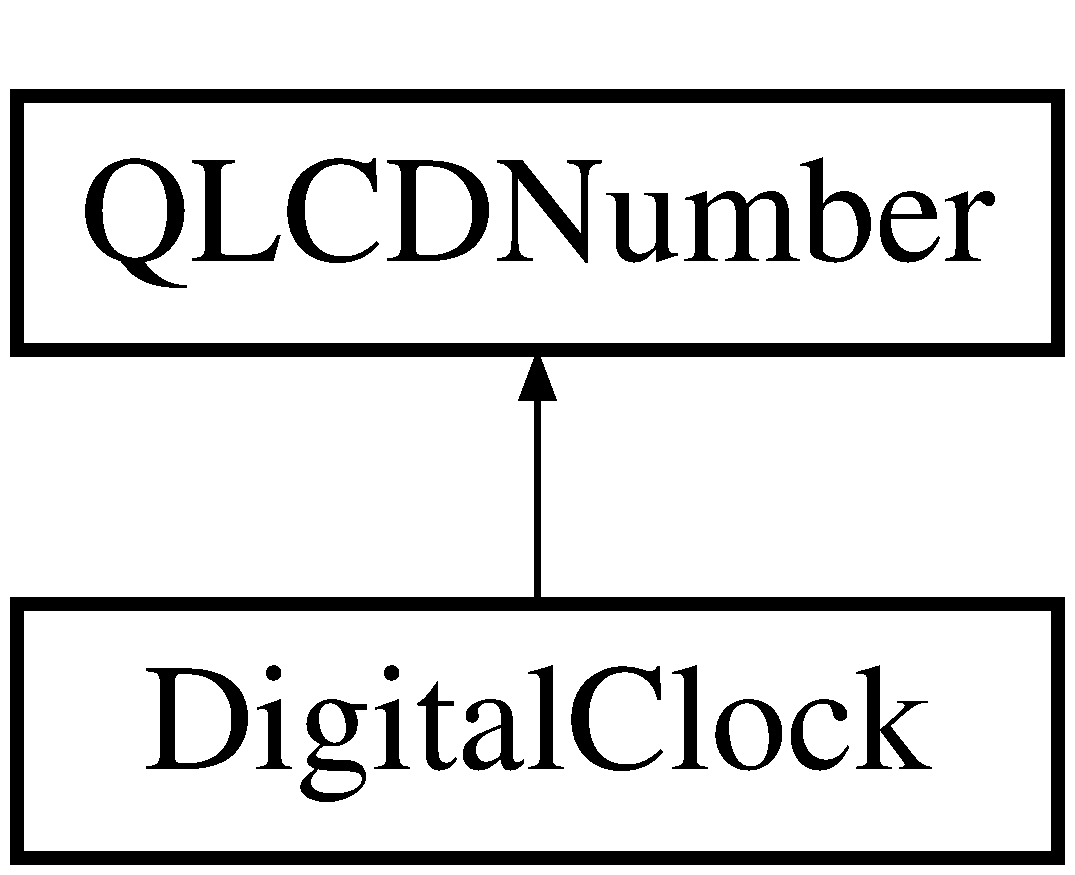
\includegraphics[height=2.000000cm]{class_digital_clock}
\end{center}
\end{figure}
\subsection*{Public Member Functions}
\begin{DoxyCompactItemize}
\item 
\mbox{\hyperlink{class_digital_clock_a1df69f177d5defdd5029ff2e6b7cb564}{Digital\+Clock}} (Q\+Widget $\ast$parent=0)
\begin{DoxyCompactList}\small\item\em Digital Clock class initializer; connects timer to digital clock to always show updated time. \end{DoxyCompactList}\end{DoxyCompactItemize}
\subsection*{Private Slots}
\begin{DoxyCompactItemize}
\item 
void \mbox{\hyperlink{class_digital_clock_a87cd1f935265a947f2ece712bffc4aaa}{show\+Time}} ()
\begin{DoxyCompactList}\small\item\em gets the current time and displays in HH\+:MM format \end{DoxyCompactList}\end{DoxyCompactItemize}


\subsection{Detailed Description}
Digital Clock class displays the current time. 

\begin{DoxyAuthor}{Author}
Meghan hannon 
\end{DoxyAuthor}


\subsection{Constructor \& Destructor Documentation}
\mbox{\Hypertarget{class_digital_clock_a1df69f177d5defdd5029ff2e6b7cb564}\label{class_digital_clock_a1df69f177d5defdd5029ff2e6b7cb564}} 
\index{Digital\+Clock@{Digital\+Clock}!Digital\+Clock@{Digital\+Clock}}
\index{Digital\+Clock@{Digital\+Clock}!Digital\+Clock@{Digital\+Clock}}
\subsubsection{\texorpdfstring{Digital\+Clock()}{DigitalClock()}}
{\footnotesize\ttfamily Digital\+Clock\+::\+Digital\+Clock (\begin{DoxyParamCaption}\item[{Q\+Widget $\ast$}]{parent = {\ttfamily 0} }\end{DoxyParamCaption})}



Digital Clock class initializer; connects timer to digital clock to always show updated time. 


\begin{DoxyParams}{Parameters}
{\em parent} & the parent widget of the digital clock \\
\hline
\end{DoxyParams}
\begin{DoxyAuthor}{Author}
Meghan Hannon 
\end{DoxyAuthor}


\subsection{Member Function Documentation}
\mbox{\Hypertarget{class_digital_clock_a87cd1f935265a947f2ece712bffc4aaa}\label{class_digital_clock_a87cd1f935265a947f2ece712bffc4aaa}} 
\index{Digital\+Clock@{Digital\+Clock}!show\+Time@{show\+Time}}
\index{show\+Time@{show\+Time}!Digital\+Clock@{Digital\+Clock}}
\subsubsection{\texorpdfstring{show\+Time}{showTime}}
{\footnotesize\ttfamily void Digital\+Clock\+::show\+Time (\begin{DoxyParamCaption}{ }\end{DoxyParamCaption})\hspace{0.3cm}{\ttfamily [private]}, {\ttfamily [slot]}}



gets the current time and displays in HH\+:MM format 

\begin{DoxyAuthor}{Author}
Meghan Hannon 
\end{DoxyAuthor}


The documentation for this class was generated from the following files\+:\begin{DoxyCompactItemize}
\item 
digitalclock.\+h\item 
digitalclock.\+cpp\end{DoxyCompactItemize}

\hypertarget{classimage}{}\section{image Class Reference}
\label{classimage}\index{image@{image}}


This class takes a given Q\+Quick\+Widget and displays an image given the absolute path.  




{\ttfamily \#include $<$image.\+h$>$}

Inheritance diagram for image\+:\begin{figure}[H]
\begin{center}
\leavevmode
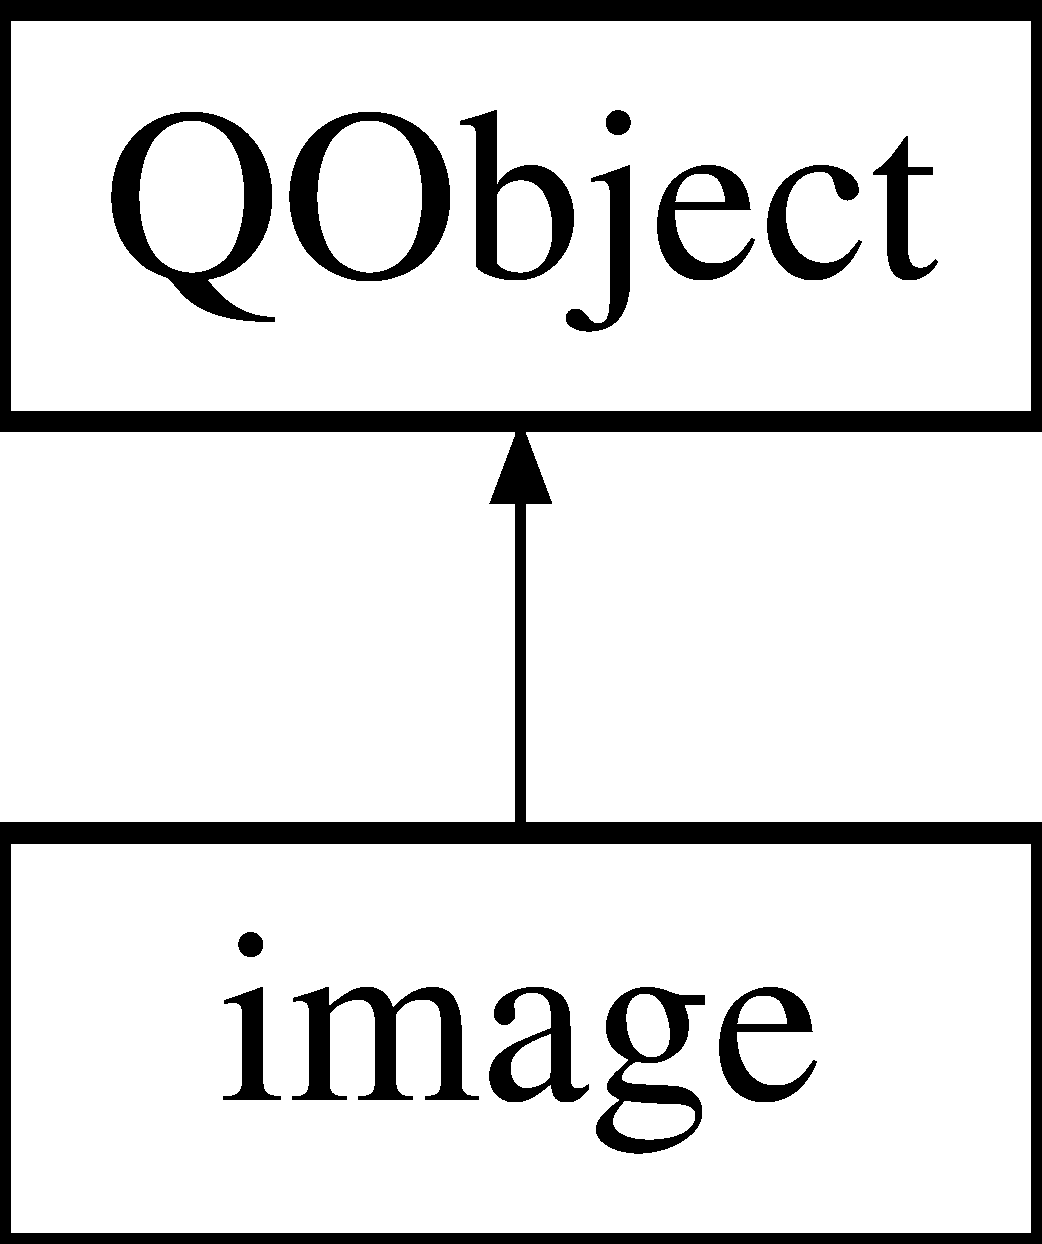
\includegraphics[height=2.000000cm]{classimage}
\end{center}
\end{figure}
\subsection*{Public Slots}
\begin{DoxyCompactItemize}
\item 
void \mbox{\hyperlink{classimage_aa5f8271e58a9264d5f6a931e6d216f8d}{update}} ()
\begin{DoxyCompactList}\small\item\em Loads the image name in the singleton class picturename to the widget\textquotesingle{}s label and displays the image or an error if no image exists. \end{DoxyCompactList}\end{DoxyCompactItemize}
\subsection*{Public Member Functions}
\begin{DoxyCompactItemize}
\item 
\mbox{\hyperlink{classimage_ab150836a04739566de187f967d657d7d}{image}} (Q\+Quick\+Widget $\ast$parent=nullptr)
\begin{DoxyCompactList}\small\item\em This class takes a given Q\+Quick\+Widget and displays an image given the absolute path. Will update on a change in picturename. \end{DoxyCompactList}\end{DoxyCompactItemize}
\subsection*{Private Attributes}
\begin{DoxyCompactItemize}
\item 
\mbox{\Hypertarget{classimage_a3a6444f79bfe79bc5af089854b157b22}\label{classimage_a3a6444f79bfe79bc5af089854b157b22}} 
Q\+Label $\ast$ {\bfseries label}
\end{DoxyCompactItemize}


\subsection{Detailed Description}
This class takes a given Q\+Quick\+Widget and displays an image given the absolute path. 

\begin{DoxyAuthor}{Author}
Stacey Gunderson, Alison Lee ~\newline
The image class displays an image using a Q\+Label 

Stacey Gunderson, Alison Lee 
\end{DoxyAuthor}


\subsection{Constructor \& Destructor Documentation}
\mbox{\Hypertarget{classimage_ab150836a04739566de187f967d657d7d}\label{classimage_ab150836a04739566de187f967d657d7d}} 
\index{image@{image}!image@{image}}
\index{image@{image}!image@{image}}
\subsubsection{\texorpdfstring{image()}{image()}}
{\footnotesize\ttfamily image\+::image (\begin{DoxyParamCaption}\item[{Q\+Quick\+Widget $\ast$}]{parent = {\ttfamily nullptr} }\end{DoxyParamCaption})\hspace{0.3cm}{\ttfamily [explicit]}}



This class takes a given Q\+Quick\+Widget and displays an image given the absolute path. Will update on a change in picturename. 

\begin{DoxyAuthor}{Author}
Stacey Gunderson, Alison Lee This class takes a given Q\+Quick\+Widget and sets up a label to call an image refresh to load the picture name 

Stacey Gunderson, Alison Lee 
\end{DoxyAuthor}


\subsection{Member Function Documentation}
\mbox{\Hypertarget{classimage_aa5f8271e58a9264d5f6a931e6d216f8d}\label{classimage_aa5f8271e58a9264d5f6a931e6d216f8d}} 
\index{image@{image}!update@{update}}
\index{update@{update}!image@{image}}
\subsubsection{\texorpdfstring{update}{update}}
{\footnotesize\ttfamily void image\+::update (\begin{DoxyParamCaption}{ }\end{DoxyParamCaption})\hspace{0.3cm}{\ttfamily [slot]}}



Loads the image name in the singleton class picturename to the widget\textquotesingle{}s label and displays the image or an error if no image exists. 

\begin{DoxyAuthor}{Author}
Stacey Gunderson, Alison Lee 
\end{DoxyAuthor}


The documentation for this class was generated from the following files\+:\begin{DoxyCompactItemize}
\item 
image.\+h\item 
image.\+cpp\end{DoxyCompactItemize}

\hypertarget{class_main_window}{}\section{Main\+Window Class Reference}
\label{class_main_window}\index{Main\+Window@{Main\+Window}}
Inheritance diagram for Main\+Window\+:\begin{figure}[H]
\begin{center}
\leavevmode
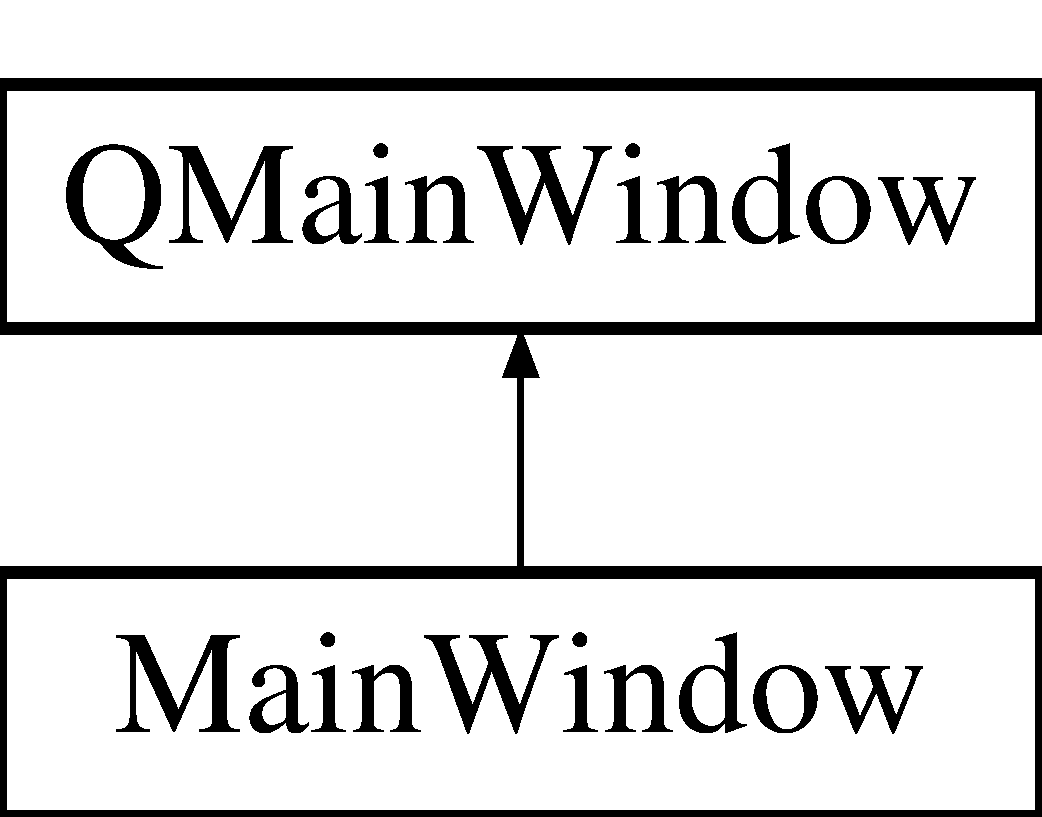
\includegraphics[height=2.000000cm]{class_main_window}
\end{center}
\end{figure}
\subsection*{Public Member Functions}
\begin{DoxyCompactItemize}
\item 
\mbox{\Hypertarget{class_main_window_a996c5a2b6f77944776856f08ec30858d}\label{class_main_window_a996c5a2b6f77944776856f08ec30858d}} 
\mbox{\hyperlink{class_main_window_a996c5a2b6f77944776856f08ec30858d}{Main\+Window}} (Q\+Widget $\ast$parent=nullptr)
\begin{DoxyCompactList}\small\item\em creates main UI Window \end{DoxyCompactList}\item 
\mbox{\Hypertarget{class_main_window_ae98d00a93bc118200eeef9f9bba1dba7}\label{class_main_window_ae98d00a93bc118200eeef9f9bba1dba7}} 
\mbox{\hyperlink{class_main_window_ae98d00a93bc118200eeef9f9bba1dba7}{$\sim$\+Main\+Window}} ()
\begin{DoxyCompactList}\small\item\em deletes UI \end{DoxyCompactList}\end{DoxyCompactItemize}
\subsection*{Private Attributes}
\begin{DoxyCompactItemize}
\item 
\mbox{\Hypertarget{class_main_window_a35466a70ed47252a0191168126a352a5}\label{class_main_window_a35466a70ed47252a0191168126a352a5}} 
Ui\+::\+Main\+Window $\ast$ {\bfseries ui}
\end{DoxyCompactItemize}


The documentation for this class was generated from the following files\+:\begin{DoxyCompactItemize}
\item 
mainwindow.\+h\item 
mainwindow.\+cpp\end{DoxyCompactItemize}

\hypertarget{classnews}{}\section{news Class Reference}
\label{classnews}\index{news@{news}}


This class takes a given parent Q\+Quick\+Widget and displays a news media blog in it.  




{\ttfamily \#include $<$news.\+h$>$}

Inheritance diagram for news\+:\begin{figure}[H]
\begin{center}
\leavevmode
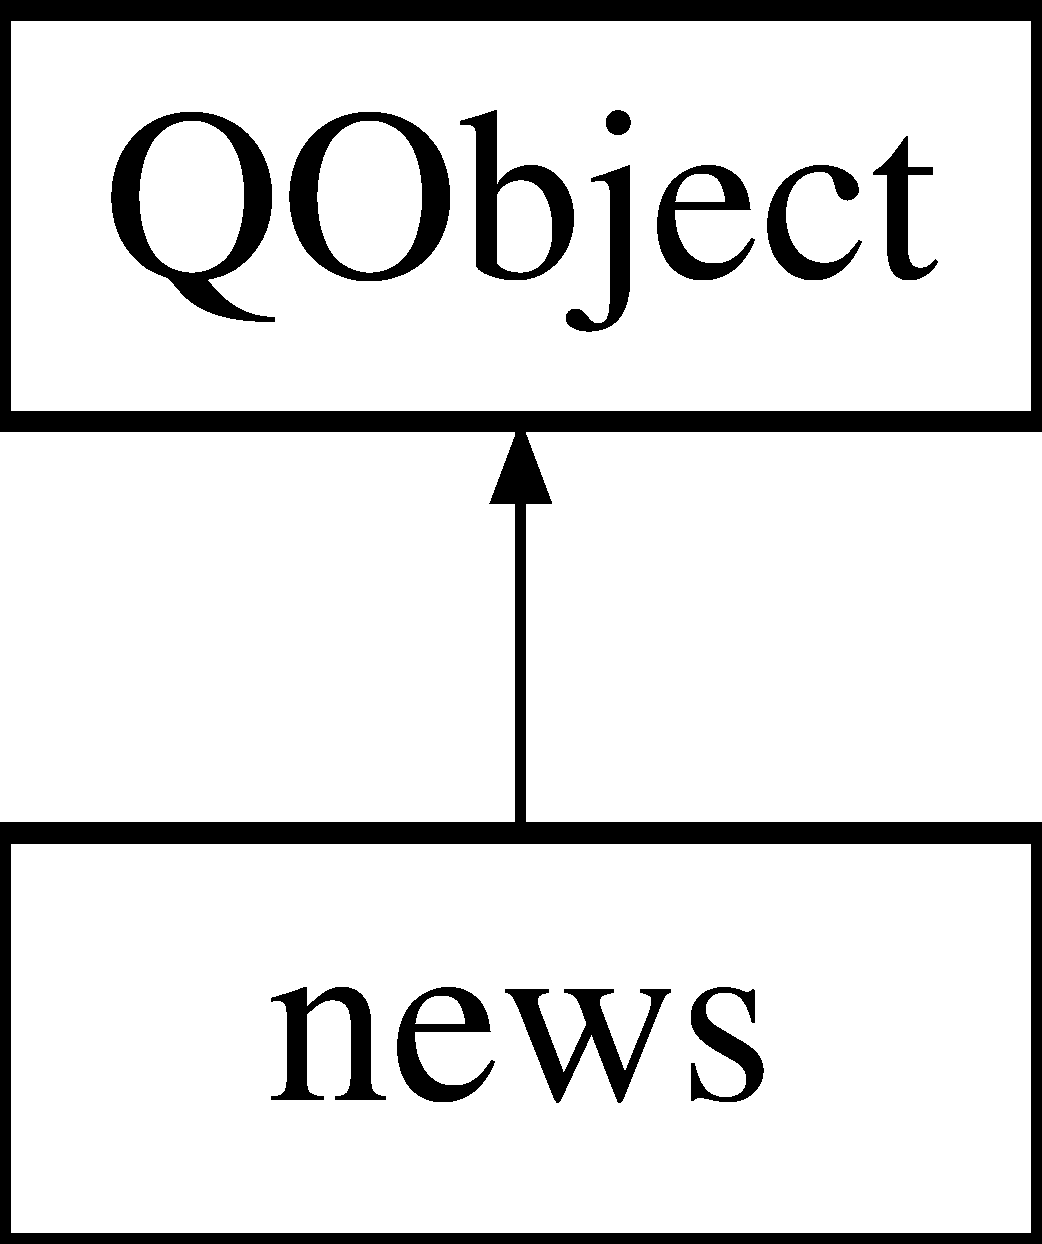
\includegraphics[height=2.000000cm]{classnews}
\end{center}
\end{figure}
\subsection*{Public Slots}
\begin{DoxyCompactItemize}
\item 
void \mbox{\hyperlink{classnews_a048f06e78e76602e4a8d2eb560bf9a23}{on\+\_\+reload}} ()
\begin{DoxyCompactList}\small\item\em This class takes a given parent Q\+Quick\+Widget and displays a news feed. \end{DoxyCompactList}\end{DoxyCompactItemize}
\subsection*{Signals}
\begin{DoxyCompactItemize}
\item 
\mbox{\Hypertarget{classnews_a81a386e5beb8547d605d862a25623310}\label{classnews_a81a386e5beb8547d605d862a25623310}} 
void {\bfseries reload} ()
\end{DoxyCompactItemize}
\subsection*{Public Member Functions}
\begin{DoxyCompactItemize}
\item 
\mbox{\hyperlink{classnews_ac5f561e7fd8a2773200bf2925208a732}{news}} (Q\+Quick\+Widget $\ast$parent=nullptr)
\begin{DoxyCompactList}\small\item\em Constructor that takes the given parent widget and displays a news media blog inside it, can be updated on button click. \end{DoxyCompactList}\end{DoxyCompactItemize}
\subsection*{Private Attributes}
\begin{DoxyCompactItemize}
\item 
\mbox{\Hypertarget{classnews_abbbded8e86c013dd7a92b810e7aea641}\label{classnews_abbbded8e86c013dd7a92b810e7aea641}} 
Q\+Web\+Engine\+View $\ast$ {\bfseries wv}
\item 
\mbox{\Hypertarget{classnews_acd7048edc8e822e30c3308f7448be600}\label{classnews_acd7048edc8e822e30c3308f7448be600}} 
Q\+Push\+Button $\ast$ {\bfseries reloadbutton}
\item 
\mbox{\Hypertarget{classnews_ab6b05e5dc5be51eccdda395f5a575a03}\label{classnews_ab6b05e5dc5be51eccdda395f5a575a03}} 
Q\+String {\bfseries stylebutton} = \char`\"{}background-\/color\+: white; color\+: black\char`\"{}
\item 
\mbox{\Hypertarget{classnews_a56769d905947c4a800d2a8a67ed9c97e}\label{classnews_a56769d905947c4a800d2a8a67ed9c97e}} 
Q\+String {\bfseries url}
\end{DoxyCompactItemize}


\subsection{Detailed Description}
This class takes a given parent Q\+Quick\+Widget and displays a news media blog in it. 

\begin{DoxyAuthor}{Author}
Stacey Gunderson, Alison Lee ~\newline
The news class inherits from Q\+Object to get access to signals and slots for updating 

Stacey Gunderson, Alison Lee 
\end{DoxyAuthor}


\subsection{Constructor \& Destructor Documentation}
\mbox{\Hypertarget{classnews_ac5f561e7fd8a2773200bf2925208a732}\label{classnews_ac5f561e7fd8a2773200bf2925208a732}} 
\index{news@{news}!news@{news}}
\index{news@{news}!news@{news}}
\subsubsection{\texorpdfstring{news()}{news()}}
{\footnotesize\ttfamily news\+::news (\begin{DoxyParamCaption}\item[{Q\+Quick\+Widget $\ast$}]{parent = {\ttfamily nullptr} }\end{DoxyParamCaption})}



Constructor that takes the given parent widget and displays a news media blog inside it, can be updated on button click. 

\begin{DoxyAuthor}{Author}
Stacey Gunderson, Alison Lee 
\end{DoxyAuthor}

\begin{DoxyParams}{Parameters}
{\em Q\+Quick\+Widget} & parent widget to display the news media blog in \\
\hline
\end{DoxyParams}


\subsection{Member Function Documentation}
\mbox{\Hypertarget{classnews_a048f06e78e76602e4a8d2eb560bf9a23}\label{classnews_a048f06e78e76602e4a8d2eb560bf9a23}} 
\index{news@{news}!on\+\_\+reload@{on\+\_\+reload}}
\index{on\+\_\+reload@{on\+\_\+reload}!news@{news}}
\subsubsection{\texorpdfstring{on\+\_\+reload}{on\_reload}}
{\footnotesize\ttfamily void news\+::on\+\_\+reload (\begin{DoxyParamCaption}{ }\end{DoxyParamCaption})\hspace{0.3cm}{\ttfamily [slot]}}



This class takes a given parent Q\+Quick\+Widget and displays a news feed. 

\begin{DoxyRefDesc}{Bug}
\item[\mbox{\hyperlink{bug__bug000001}{Bug}}]May throw warnings and errors to console about missing sync tokens, will not crash Everything works nicely on the front end \end{DoxyRefDesc}
\begin{DoxyAuthor}{Author}
Stacey Gunderson, Alison Lee Upon button click signal, reloads the url to refresh what is on the page 

Stacey Gunderson, Alison Lee 
\end{DoxyAuthor}
\begin{DoxyReturn}{Returns}
void 
\end{DoxyReturn}


The documentation for this class was generated from the following files\+:\begin{DoxyCompactItemize}
\item 
news.\+h\item 
news.\+cpp\end{DoxyCompactItemize}

\hypertarget{classpicturename}{}\section{picturename Class Reference}
\label{classpicturename}\index{picturename@{picturename}}


A singleton design that holds a single given Q\+String object for a picture name.  




{\ttfamily \#include $<$picturename.\+h$>$}

Inheritance diagram for picturename\+:\begin{figure}[H]
\begin{center}
\leavevmode
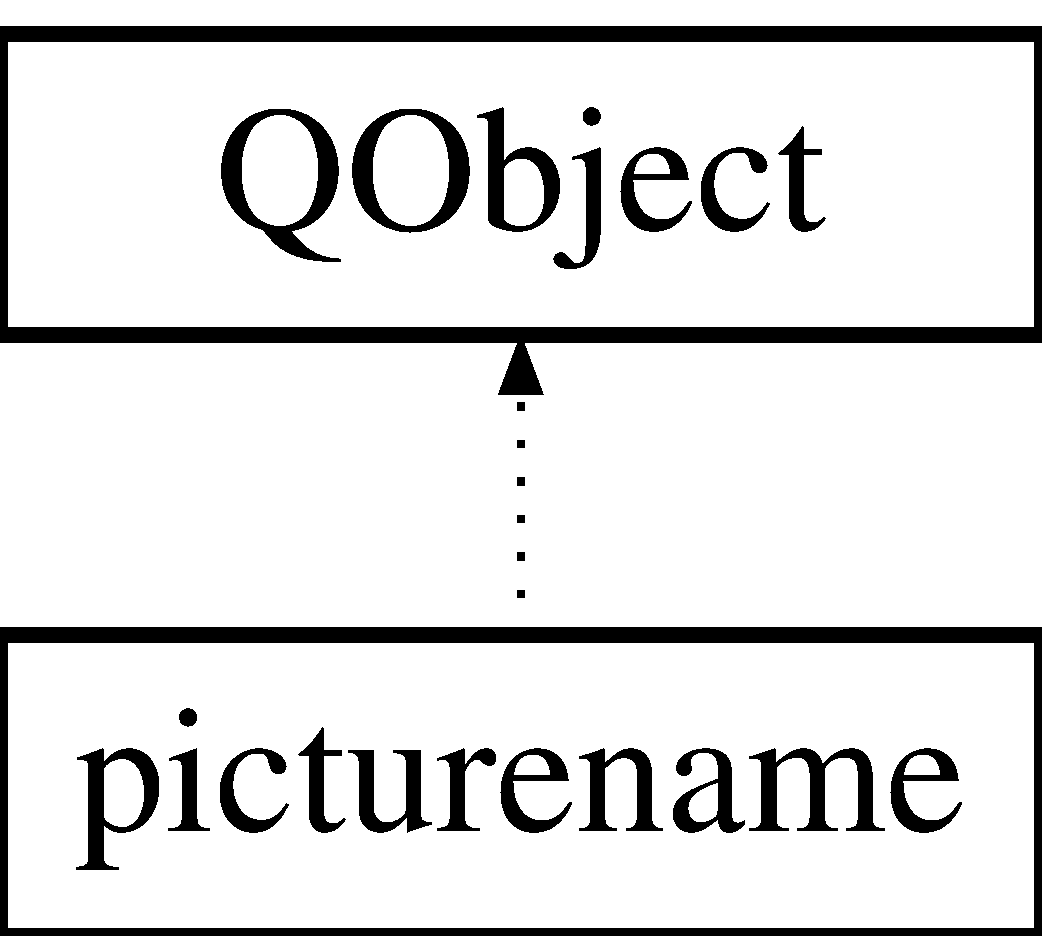
\includegraphics[height=2.000000cm]{classpicturename}
\end{center}
\end{figure}
\subsection*{Signals}
\begin{DoxyCompactItemize}
\item 
\mbox{\Hypertarget{classpicturename_a82cfb404225352e4148ebb462ad74762}\label{classpicturename_a82cfb404225352e4148ebb462ad74762}} 
void {\bfseries notify} ()
\end{DoxyCompactItemize}
\subsection*{Public Member Functions}
\begin{DoxyCompactItemize}
\item 
Q\+String \mbox{\hyperlink{classpicturename_a6b2c3caa683878aa5f95b9276502a8ae}{get\+\_\+picture}} ()
\begin{DoxyCompactList}\small\item\em Returns the Q\+String with the name of the picture. \end{DoxyCompactList}\item 
void \mbox{\hyperlink{classpicturename_a4b95f1c195e8ef08203f3e3204db5bfe}{add\+\_\+observer}} (\mbox{\hyperlink{classimage}{image}} $\ast$)
\begin{DoxyCompactList}\small\item\em Adds an observer to the list, and creates a signal connection. \end{DoxyCompactList}\item 
void \mbox{\hyperlink{classpicturename_ae4b0e336db224b42756d00dc2c8d67ba}{remove\+\_\+observer}} (\mbox{\hyperlink{classimage}{image}} $\ast$)
\begin{DoxyCompactList}\small\item\em Removes an observer from the list. \end{DoxyCompactList}\item 
void \mbox{\hyperlink{classpicturename_ab96020b531c8e2c852ea4bc17969e36c}{set\+\_\+picture}} (Q\+String)
\begin{DoxyCompactList}\small\item\em Sets the Q\+String for the picture name to the given Q\+String and notifies observers. \end{DoxyCompactList}\end{DoxyCompactItemize}
\subsection*{Static Public Member Functions}
\begin{DoxyCompactItemize}
\item 
static \mbox{\hyperlink{classpicturename}{picturename}} \& \mbox{\hyperlink{classpicturename_a2447735d7a01afd95bceadcd5cfc28f2}{instance}} ()
\begin{DoxyCompactList}\small\item\em Returns a pointer to a singleton instance of picturename, creates one if it does not exist. \end{DoxyCompactList}\end{DoxyCompactItemize}
\subsection*{Protected Member Functions}
\begin{DoxyCompactItemize}
\item 
\mbox{\hyperlink{classpicturename_a446962c869c6f39fd01688d94f9cde1b}{picturename}} ()
\begin{DoxyCompactList}\small\item\em Creates an instance of picturename, set aurora as default image. \end{DoxyCompactList}\end{DoxyCompactItemize}
\subsection*{Private Member Functions}
\begin{DoxyCompactItemize}
\item 
\mbox{\Hypertarget{classpicturename_af440f412d5850406ca92eac1ca7f827d}\label{classpicturename_af440f412d5850406ca92eac1ca7f827d}} 
{\bfseries picturename} (\mbox{\hyperlink{classpicturename}{picturename}} \&other)
\item 
\mbox{\Hypertarget{classpicturename_ab392e401bcbfd809e1fe221105e92b13}\label{classpicturename_ab392e401bcbfd809e1fe221105e92b13}} 
\mbox{\hyperlink{classpicturename}{picturename}} \& {\bfseries operator=} (\mbox{\hyperlink{classpicturename}{picturename}} \&other)
\end{DoxyCompactItemize}
\subsection*{Private Attributes}
\begin{DoxyCompactItemize}
\item 
\mbox{\Hypertarget{classpicturename_af389638c5b4dbf88569aeb5f2e173ffd}\label{classpicturename_af389638c5b4dbf88569aeb5f2e173ffd}} 
Q\+String {\bfseries picturelink}
\item 
\mbox{\Hypertarget{classpicturename_a6fe14cb9fa6bde776f9ddf0f1904fbb3}\label{classpicturename_a6fe14cb9fa6bde776f9ddf0f1904fbb3}} 
Q\+List$<$ \mbox{\hyperlink{classimage}{image}} $\ast$ $>$ {\bfseries observers}
\end{DoxyCompactItemize}
\subsection*{Static Private Attributes}
\begin{DoxyCompactItemize}
\item 
static \mbox{\hyperlink{classpicturename}{picturename}} $\ast$ \mbox{\hyperlink{classpicturename_ab2f5e20595601416bf9f3e1b65a547d4}{\+\_\+instance}} = N\+U\+LL
\begin{DoxyCompactList}\small\item\em A singleton design that holds a single given Q\+String object for a picture name. \end{DoxyCompactList}\end{DoxyCompactItemize}


\subsection{Detailed Description}
A singleton design that holds a single given Q\+String object for a picture name. 

\begin{DoxyAuthor}{Author}
Stacey Gunderson, Alison Lee 
\end{DoxyAuthor}


\subsection{Constructor \& Destructor Documentation}
\mbox{\Hypertarget{classpicturename_a446962c869c6f39fd01688d94f9cde1b}\label{classpicturename_a446962c869c6f39fd01688d94f9cde1b}} 
\index{picturename@{picturename}!picturename@{picturename}}
\index{picturename@{picturename}!picturename@{picturename}}
\subsubsection{\texorpdfstring{picturename()}{picturename()}}
{\footnotesize\ttfamily picturename\+::picturename (\begin{DoxyParamCaption}{ }\end{DoxyParamCaption})\hspace{0.3cm}{\ttfamily [protected]}}



Creates an instance of picturename, set aurora as default image. 

\begin{DoxyAuthor}{Author}
Stacey Gunderson, Alison Lee 
\end{DoxyAuthor}


\subsection{Member Function Documentation}
\mbox{\Hypertarget{classpicturename_a4b95f1c195e8ef08203f3e3204db5bfe}\label{classpicturename_a4b95f1c195e8ef08203f3e3204db5bfe}} 
\index{picturename@{picturename}!add\+\_\+observer@{add\+\_\+observer}}
\index{add\+\_\+observer@{add\+\_\+observer}!picturename@{picturename}}
\subsubsection{\texorpdfstring{add\+\_\+observer()}{add\_observer()}}
{\footnotesize\ttfamily void picturename\+::add\+\_\+observer (\begin{DoxyParamCaption}\item[{\mbox{\hyperlink{classimage}{image}} $\ast$}]{obj }\end{DoxyParamCaption})}



Adds an observer to the list, and creates a signal connection. 

\begin{DoxyAuthor}{Author}
Stacey Gunderson, Alison Lee 
\end{DoxyAuthor}
\mbox{\Hypertarget{classpicturename_a6b2c3caa683878aa5f95b9276502a8ae}\label{classpicturename_a6b2c3caa683878aa5f95b9276502a8ae}} 
\index{picturename@{picturename}!get\+\_\+picture@{get\+\_\+picture}}
\index{get\+\_\+picture@{get\+\_\+picture}!picturename@{picturename}}
\subsubsection{\texorpdfstring{get\+\_\+picture()}{get\_picture()}}
{\footnotesize\ttfamily Q\+String picturename\+::get\+\_\+picture (\begin{DoxyParamCaption}{ }\end{DoxyParamCaption})}



Returns the Q\+String with the name of the picture. 

\begin{DoxyAuthor}{Author}
Stacey Gunderson, Alison Lee 
\end{DoxyAuthor}
\mbox{\Hypertarget{classpicturename_a2447735d7a01afd95bceadcd5cfc28f2}\label{classpicturename_a2447735d7a01afd95bceadcd5cfc28f2}} 
\index{picturename@{picturename}!instance@{instance}}
\index{instance@{instance}!picturename@{picturename}}
\subsubsection{\texorpdfstring{instance()}{instance()}}
{\footnotesize\ttfamily \mbox{\hyperlink{classpicturename}{picturename}} \& picturename\+::instance (\begin{DoxyParamCaption}{ }\end{DoxyParamCaption})\hspace{0.3cm}{\ttfamily [static]}}



Returns a pointer to a singleton instance of picturename, creates one if it does not exist. 

\begin{DoxyAuthor}{Author}
Stacey Gunderson, Alison Lee 
\end{DoxyAuthor}
\begin{DoxyReturn}{Returns}
the pointer to the instance of picturename 
\end{DoxyReturn}
\mbox{\Hypertarget{classpicturename_ae4b0e336db224b42756d00dc2c8d67ba}\label{classpicturename_ae4b0e336db224b42756d00dc2c8d67ba}} 
\index{picturename@{picturename}!remove\+\_\+observer@{remove\+\_\+observer}}
\index{remove\+\_\+observer@{remove\+\_\+observer}!picturename@{picturename}}
\subsubsection{\texorpdfstring{remove\+\_\+observer()}{remove\_observer()}}
{\footnotesize\ttfamily void picturename\+::remove\+\_\+observer (\begin{DoxyParamCaption}\item[{\mbox{\hyperlink{classimage}{image}} $\ast$}]{obj }\end{DoxyParamCaption})}



Removes an observer from the list. 

\begin{DoxyAuthor}{Author}
Stacey Gunderson, Alison Lee 
\end{DoxyAuthor}
\mbox{\Hypertarget{classpicturename_ab96020b531c8e2c852ea4bc17969e36c}\label{classpicturename_ab96020b531c8e2c852ea4bc17969e36c}} 
\index{picturename@{picturename}!set\+\_\+picture@{set\+\_\+picture}}
\index{set\+\_\+picture@{set\+\_\+picture}!picturename@{picturename}}
\subsubsection{\texorpdfstring{set\+\_\+picture()}{set\_picture()}}
{\footnotesize\ttfamily void picturename\+::set\+\_\+picture (\begin{DoxyParamCaption}\item[{Q\+String}]{link }\end{DoxyParamCaption})}



Sets the Q\+String for the picture name to the given Q\+String and notifies observers. 

\begin{DoxyAuthor}{Author}
Stacey Gunderson, Alison Lee 
\end{DoxyAuthor}


\subsection{Member Data Documentation}
\mbox{\Hypertarget{classpicturename_ab2f5e20595601416bf9f3e1b65a547d4}\label{classpicturename_ab2f5e20595601416bf9f3e1b65a547d4}} 
\index{picturename@{picturename}!\+\_\+instance@{\+\_\+instance}}
\index{\+\_\+instance@{\+\_\+instance}!picturename@{picturename}}
\subsubsection{\texorpdfstring{\+\_\+instance}{\_instance}}
{\footnotesize\ttfamily \mbox{\hyperlink{classpicturename}{picturename}} $\ast$ picturename\+::\+\_\+instance = N\+U\+LL\hspace{0.3cm}{\ttfamily [static]}, {\ttfamily [private]}}



A singleton design that holds a single given Q\+String object for a picture name. 

\begin{DoxyAuthor}{Author}
Stacey Gunderson, Alison Lee 
\end{DoxyAuthor}


The documentation for this class was generated from the following files\+:\begin{DoxyCompactItemize}
\item 
picturename.\+h\item 
picturename.\+cpp\end{DoxyCompactItemize}

\hypertarget{classsocial}{}\section{social Class Reference}
\label{classsocial}\index{social@{social}}


This class takes a given parent Q\+Quick\+Widget and displays a social media blog in it.  




{\ttfamily \#include $<$social.\+h$>$}

Inheritance diagram for social\+:\begin{figure}[H]
\begin{center}
\leavevmode
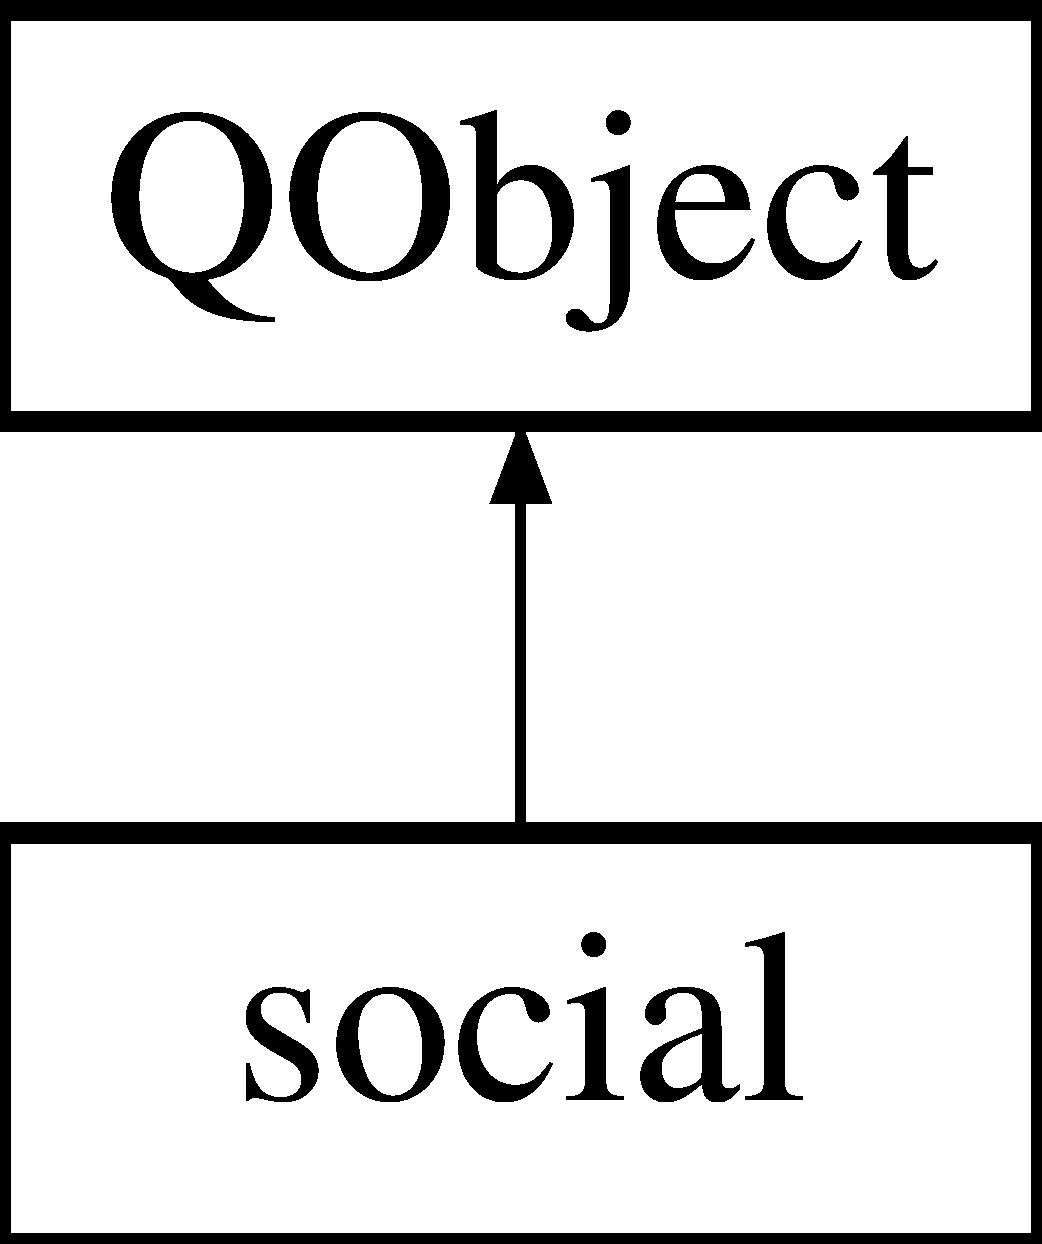
\includegraphics[height=2.000000cm]{classsocial}
\end{center}
\end{figure}
\subsection*{Public Slots}
\begin{DoxyCompactItemize}
\item 
void \mbox{\hyperlink{classsocial_aed7a46c6bae233cd68a61aefc8ba3915}{on\+\_\+reload}} ()
\begin{DoxyCompactList}\small\item\em This class takes a given parent Q\+Quick\+Widget and displays a social media blog in it. \end{DoxyCompactList}\end{DoxyCompactItemize}
\subsection*{Signals}
\begin{DoxyCompactItemize}
\item 
\mbox{\Hypertarget{classsocial_a000ed24b8b1e7abfc04dce3b76139fcd}\label{classsocial_a000ed24b8b1e7abfc04dce3b76139fcd}} 
void {\bfseries reload} ()
\end{DoxyCompactItemize}
\subsection*{Public Member Functions}
\begin{DoxyCompactItemize}
\item 
\mbox{\hyperlink{classsocial_ae8c36ee55976d5b9fb5f7738be4ed2c1}{social}} (Q\+Quick\+Widget $\ast$parent=nullptr)
\begin{DoxyCompactList}\small\item\em Constructor that takes the given parent widget and displays a social media blog inside it, can be updated on button click. \end{DoxyCompactList}\end{DoxyCompactItemize}
\subsection*{Private Attributes}
\begin{DoxyCompactItemize}
\item 
\mbox{\Hypertarget{classsocial_af3bc85613901d458ce579967d5f1fb38}\label{classsocial_af3bc85613901d458ce579967d5f1fb38}} 
Q\+Web\+Engine\+View $\ast$ {\bfseries wv}
\item 
\mbox{\Hypertarget{classsocial_ad4e1926a47c20d06b0ee910ab298d9a9}\label{classsocial_ad4e1926a47c20d06b0ee910ab298d9a9}} 
Q\+Push\+Button $\ast$ {\bfseries reloadbutton}
\item 
\mbox{\Hypertarget{classsocial_a16d2a524d4366696b9cff6d04426aa63}\label{classsocial_a16d2a524d4366696b9cff6d04426aa63}} 
const Q\+String {\bfseries style} = \char`\"{}background-\/color\+: \#A3\+C1\+DA; color\+: white;\char`\"{}
\item 
\mbox{\Hypertarget{classsocial_ae4ed1fe9e3a3dbd9492ad2689509228e}\label{classsocial_ae4ed1fe9e3a3dbd9492ad2689509228e}} 
Q\+String {\bfseries stylebutton} = \char`\"{}background-\/color\+: white; color\+: black\char`\"{}
\item 
\mbox{\Hypertarget{classsocial_abaae965357c4daea14964c1c5237a9d4}\label{classsocial_abaae965357c4daea14964c1c5237a9d4}} 
Q\+Line\+Edit $\ast$ {\bfseries urlbox}
\item 
\mbox{\Hypertarget{classsocial_abadd3b592cd9a28b0201595f4c448ffc}\label{classsocial_abadd3b592cd9a28b0201595f4c448ffc}} 
Q\+String {\bfseries url}
\end{DoxyCompactItemize}


\subsection{Detailed Description}
This class takes a given parent Q\+Quick\+Widget and displays a social media blog in it. 

\begin{DoxyAuthor}{Author}
Stacey Gunderson, Alison Lee ~\newline
The social class inherits from Q\+Object to get access to signals and slots for updating 

Stacey Gunderson, Alison Lee 
\end{DoxyAuthor}


\subsection{Constructor \& Destructor Documentation}
\mbox{\Hypertarget{classsocial_ae8c36ee55976d5b9fb5f7738be4ed2c1}\label{classsocial_ae8c36ee55976d5b9fb5f7738be4ed2c1}} 
\index{social@{social}!social@{social}}
\index{social@{social}!social@{social}}
\subsubsection{\texorpdfstring{social()}{social()}}
{\footnotesize\ttfamily social\+::social (\begin{DoxyParamCaption}\item[{Q\+Quick\+Widget $\ast$}]{parent = {\ttfamily nullptr} }\end{DoxyParamCaption})}



Constructor that takes the given parent widget and displays a social media blog inside it, can be updated on button click. 

\begin{DoxyAuthor}{Author}
Stacey Gunderson, Alison Lee 
\end{DoxyAuthor}

\begin{DoxyParams}{Parameters}
{\em Q\+Quick\+Widget} & parent widget to display the social media blog in \\
\hline
\end{DoxyParams}


\subsection{Member Function Documentation}
\mbox{\Hypertarget{classsocial_aed7a46c6bae233cd68a61aefc8ba3915}\label{classsocial_aed7a46c6bae233cd68a61aefc8ba3915}} 
\index{social@{social}!on\+\_\+reload@{on\+\_\+reload}}
\index{on\+\_\+reload@{on\+\_\+reload}!social@{social}}
\subsubsection{\texorpdfstring{on\+\_\+reload}{on\_reload}}
{\footnotesize\ttfamily void social\+::on\+\_\+reload (\begin{DoxyParamCaption}{ }\end{DoxyParamCaption})\hspace{0.3cm}{\ttfamily [slot]}}



This class takes a given parent Q\+Quick\+Widget and displays a social media blog in it. 

\begin{DoxyRefDesc}{Bug}
\item[\mbox{\hyperlink{bug__bug000002}{Bug}}]Will throw warnings and errors to console about missing sync tokens?? Everything works nicely on the front end \end{DoxyRefDesc}
\begin{DoxyAuthor}{Author}
Stacey Gunderson, Alison Lee Upon button click signal, reloads the url to refresh what is on the page 

Stacey Gunderson, Alison Lee 
\end{DoxyAuthor}
\begin{DoxyReturn}{Returns}
void 
\end{DoxyReturn}


The documentation for this class was generated from the following files\+:\begin{DoxyCompactItemize}
\item 
social.\+h\item 
social.\+cpp\end{DoxyCompactItemize}

\hypertarget{classweatherpanel}{}\section{weatherpanel Class Reference}
\label{classweatherpanel}\index{weatherpanel@{weatherpanel}}
Inheritance diagram for weatherpanel\+:\begin{figure}[H]
\begin{center}
\leavevmode
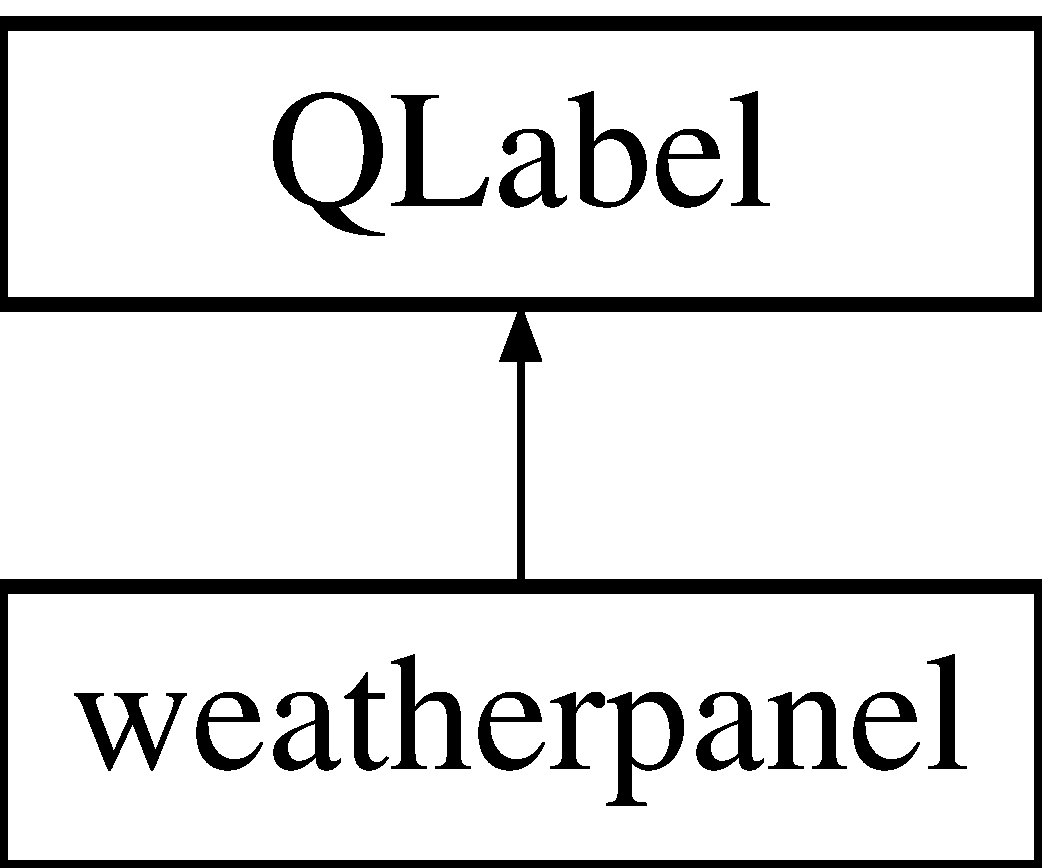
\includegraphics[height=2.000000cm]{classweatherpanel}
\end{center}
\end{figure}
\subsection*{Public Member Functions}
\begin{DoxyCompactItemize}
\item 
int \mbox{\hyperlink{classweatherpanel_a45e1d05896ce57be8a2485f7559c4276}{get\+Weather\+ID}} ()
\begin{DoxyCompactList}\small\item\em returns an integer representing the type of weather \end{DoxyCompactList}\item 
void \mbox{\hyperlink{classweatherpanel_adcfb5683fa421ee6b45b775ca3b6c5ae}{set\+Weather\+ID}} (int to\+Set)
\begin{DoxyCompactList}\small\item\em sets weather\+ID to an integer representing the type of weather \end{DoxyCompactList}\item 
\mbox{\hyperlink{classweatherpanel_a4f24bc46cb882bf72f7712a6aca35fbb}{weatherpanel}} (Q\+Quick\+Widget $\ast$parent=0)
\begin{DoxyCompactList}\small\item\em this class takes a Q\+Quick\+Widget, adds a Q\+Label to it, then displays todays weather within that Q\+Label \end{DoxyCompactList}\item 
Q\+String \mbox{\hyperlink{classweatherpanel_a6f90f234561aa11f374fbd6f89e4c02b}{get\+ID}} ()
\begin{DoxyCompactList}\small\item\em returns a Q\+String holding the openweathermaps api key \end{DoxyCompactList}\item 
void \mbox{\hyperlink{classweatherpanel_aa289deea2382682a44450048c5d8dafb}{set\+Weather}} (Q\+String weather\+In)
\begin{DoxyCompactList}\small\item\em sets weather to a Q\+String describing the weather \end{DoxyCompactList}\item 
void \mbox{\hyperlink{classweatherpanel_a3869138bae14bb7223e78541ddb45ae9}{set\+Temp}} (Q\+String temp\+In)
\begin{DoxyCompactList}\small\item\em sets temperature to a Q\+String describing the temperature \end{DoxyCompactList}\item 
Q\+String \mbox{\hyperlink{classweatherpanel_af8d593a8bc328ea0614f9bfb3ddf4f08}{get\+Weather}} ()
\begin{DoxyCompactList}\small\item\em returns a Q\+String describing the weather \end{DoxyCompactList}\item 
Q\+String \mbox{\hyperlink{classweatherpanel_a56fe31e2484d3266b9b039eaec58da7d}{get\+Temp}} ()
\begin{DoxyCompactList}\small\item\em returns a Q\+String describing the temperature \end{DoxyCompactList}\item 
void \mbox{\hyperlink{classweatherpanel_a8c4de1853c738dcf431f33a7a3ac56e4}{update\+Text}} ()
\begin{DoxyCompactList}\small\item\em converts the data to a string then sets the Q\+Labels text to this string \end{DoxyCompactList}\end{DoxyCompactItemize}
\subsection*{Public Attributes}
\begin{DoxyCompactItemize}
\item 
\mbox{\Hypertarget{classweatherpanel_a8fad815741f5d5047e6d0c337a1016f7}\label{classweatherpanel_a8fad815741f5d5047e6d0c337a1016f7}} 
Q\+String {\bfseries w\+To\+Image}
\item 
\mbox{\Hypertarget{classweatherpanel_a391826b3d7f3df11c41df7c182639084}\label{classweatherpanel_a391826b3d7f3df11c41df7c182639084}} 
int {\bfseries weather\+ID}
\item 
\mbox{\Hypertarget{classweatherpanel_ae3b988537592d93f7b3e188e3ff96ca1}\label{classweatherpanel_ae3b988537592d93f7b3e188e3ff96ca1}} 
Q\+String {\bfseries city}
\item 
\mbox{\Hypertarget{classweatherpanel_ad53cf408c768382d7f6f5471f1f3f6a9}\label{classweatherpanel_ad53cf408c768382d7f6f5471f1f3f6a9}} 
Q\+Network\+Access\+Manager $\ast$ {\bfseries nam}
\item 
\mbox{\Hypertarget{classweatherpanel_aaaa5cb24a09525e123ef0b2f624d2d0f}\label{classweatherpanel_aaaa5cb24a09525e123ef0b2f624d2d0f}} 
Q\+Network\+Session $\ast$ {\bfseries ns}
\item 
\mbox{\Hypertarget{classweatherpanel_a0db73d897f7290fa37f3e3af183a3587}\label{classweatherpanel_a0db73d897f7290fa37f3e3af183a3587}} 
Q\+String {\bfseries app\+ID}
\end{DoxyCompactItemize}
\subsection*{Private Slots}
\begin{DoxyCompactItemize}
\item 
void \mbox{\hyperlink{classweatherpanel_a212139bb98a83e8c52b30bbe786b8bb1}{pull\+Weather}} ()
\begin{DoxyCompactList}\small\item\em connects to openweathermaps api and queries for the weather data in J\+S\+ON format, calls data\+To\+Vars to save this info \end{DoxyCompactList}\end{DoxyCompactItemize}
\subsection*{Private Member Functions}
\begin{DoxyCompactItemize}
\item 
void \mbox{\hyperlink{classweatherpanel_a56353d725e339accc2952eda96d65907}{update\+Image}} ()
\begin{DoxyCompactList}\small\item\em Determines a background picture based on weather\+ID, sets the picture to the background. \end{DoxyCompactList}\item 
void \mbox{\hyperlink{classweatherpanel_a5a3f8862f3f1ae01783a3e0bc084ba69}{data\+To\+Vars}} (Q\+Network\+Reply $\ast$netreply)
\begin{DoxyCompactList}\small\item\em converts the raw data to useful variables \end{DoxyCompactList}\item 
Q\+String \mbox{\hyperlink{classweatherpanel_aa060e2d25c499b202688fdb0ed2e51f0}{KtoC}} (double temp)
\begin{DoxyCompactList}\small\item\em converts kelvin to celcius and then returns as string \end{DoxyCompactList}\end{DoxyCompactItemize}
\subsection*{Private Attributes}
\begin{DoxyCompactItemize}
\item 
\mbox{\Hypertarget{classweatherpanel_a03b9e1f4ca93f6ffb835ed19c3645d91}\label{classweatherpanel_a03b9e1f4ca93f6ffb835ed19c3645d91}} 
Q\+String {\bfseries weather}
\item 
\mbox{\Hypertarget{classweatherpanel_ab2c38c795e09f961485bef0c2f36165c}\label{classweatherpanel_ab2c38c795e09f961485bef0c2f36165c}} 
Q\+String {\bfseries temperature}
\end{DoxyCompactItemize}


\subsection{Constructor \& Destructor Documentation}
\mbox{\Hypertarget{classweatherpanel_a4f24bc46cb882bf72f7712a6aca35fbb}\label{classweatherpanel_a4f24bc46cb882bf72f7712a6aca35fbb}} 
\index{weatherpanel@{weatherpanel}!weatherpanel@{weatherpanel}}
\index{weatherpanel@{weatherpanel}!weatherpanel@{weatherpanel}}
\subsubsection{\texorpdfstring{weatherpanel()}{weatherpanel()}}
{\footnotesize\ttfamily weatherpanel\+::weatherpanel (\begin{DoxyParamCaption}\item[{Q\+Quick\+Widget $\ast$}]{parent = {\ttfamily 0} }\end{DoxyParamCaption})}



this class takes a Q\+Quick\+Widget, adds a Q\+Label to it, then displays todays weather within that Q\+Label 

\begin{DoxyAuthor}{Author}
Thomas Grummett powered by Open Weather Maps\+: openweathermaps.\+org Constructor takes a Q\+Quick\+Widget and adds the weather display to it 
\end{DoxyAuthor}

\begin{DoxyParams}{Parameters}
{\em Q\+Quick\+Widget} & parent to display the weather in \\
\hline
\end{DoxyParams}
\begin{DoxyAuthor}{Author}
Thomas Grummett 
\end{DoxyAuthor}
make sure we have an active network session

set london as default

tell the system we want network

connect timer in order to pull the weather every 5 mins 

\subsection{Member Function Documentation}
\mbox{\Hypertarget{classweatherpanel_a5a3f8862f3f1ae01783a3e0bc084ba69}\label{classweatherpanel_a5a3f8862f3f1ae01783a3e0bc084ba69}} 
\index{weatherpanel@{weatherpanel}!data\+To\+Vars@{data\+To\+Vars}}
\index{data\+To\+Vars@{data\+To\+Vars}!weatherpanel@{weatherpanel}}
\subsubsection{\texorpdfstring{data\+To\+Vars()}{dataToVars()}}
{\footnotesize\ttfamily void weatherpanel\+::data\+To\+Vars (\begin{DoxyParamCaption}\item[{Q\+Network\+Reply $\ast$}]{netreply }\end{DoxyParamCaption})\hspace{0.3cm}{\ttfamily [private]}}



converts the raw data to useful variables 


\begin{DoxyParams}{Parameters}
{\em netreply} & is the reply for a query to openweathermaps api \\
\hline
\end{DoxyParams}
\begin{DoxyAuthor}{Author}
Thomas Grummett 
\end{DoxyAuthor}
pull weather data

pull temperature

update Q\+Label \mbox{\Hypertarget{classweatherpanel_a6f90f234561aa11f374fbd6f89e4c02b}\label{classweatherpanel_a6f90f234561aa11f374fbd6f89e4c02b}} 
\index{weatherpanel@{weatherpanel}!get\+ID@{get\+ID}}
\index{get\+ID@{get\+ID}!weatherpanel@{weatherpanel}}
\subsubsection{\texorpdfstring{get\+I\+D()}{getID()}}
{\footnotesize\ttfamily Q\+String weatherpanel\+::get\+ID (\begin{DoxyParamCaption}{ }\end{DoxyParamCaption})}



returns a Q\+String holding the openweathermaps api key 

\begin{DoxyReturn}{Returns}
Q\+String app\+ID that holds the api key 
\end{DoxyReturn}
\begin{DoxyAuthor}{Author}
Thomas Grummett 
\end{DoxyAuthor}
\mbox{\Hypertarget{classweatherpanel_a56fe31e2484d3266b9b039eaec58da7d}\label{classweatherpanel_a56fe31e2484d3266b9b039eaec58da7d}} 
\index{weatherpanel@{weatherpanel}!get\+Temp@{get\+Temp}}
\index{get\+Temp@{get\+Temp}!weatherpanel@{weatherpanel}}
\subsubsection{\texorpdfstring{get\+Temp()}{getTemp()}}
{\footnotesize\ttfamily Q\+String weatherpanel\+::get\+Temp (\begin{DoxyParamCaption}{ }\end{DoxyParamCaption})}



returns a Q\+String describing the temperature 

\begin{DoxyReturn}{Returns}
Q\+String temperature that describes the temperature 
\end{DoxyReturn}
\begin{DoxyAuthor}{Author}
Thomas Grummett 
\end{DoxyAuthor}
\mbox{\Hypertarget{classweatherpanel_af8d593a8bc328ea0614f9bfb3ddf4f08}\label{classweatherpanel_af8d593a8bc328ea0614f9bfb3ddf4f08}} 
\index{weatherpanel@{weatherpanel}!get\+Weather@{get\+Weather}}
\index{get\+Weather@{get\+Weather}!weatherpanel@{weatherpanel}}
\subsubsection{\texorpdfstring{get\+Weather()}{getWeather()}}
{\footnotesize\ttfamily Q\+String weatherpanel\+::get\+Weather (\begin{DoxyParamCaption}{ }\end{DoxyParamCaption})}



returns a Q\+String describing the weather 

\begin{DoxyReturn}{Returns}
Q\+String weather that describes the weather 
\end{DoxyReturn}
\begin{DoxyAuthor}{Author}
Thomas Grummett 
\end{DoxyAuthor}
\mbox{\Hypertarget{classweatherpanel_a45e1d05896ce57be8a2485f7559c4276}\label{classweatherpanel_a45e1d05896ce57be8a2485f7559c4276}} 
\index{weatherpanel@{weatherpanel}!get\+Weather\+ID@{get\+Weather\+ID}}
\index{get\+Weather\+ID@{get\+Weather\+ID}!weatherpanel@{weatherpanel}}
\subsubsection{\texorpdfstring{get\+Weather\+I\+D()}{getWeatherID()}}
{\footnotesize\ttfamily int weatherpanel\+::get\+Weather\+ID (\begin{DoxyParamCaption}{ }\end{DoxyParamCaption})}



returns an integer representing the type of weather 

\begin{DoxyReturn}{Returns}
integer weather\+ID that represents thet type of weather 
\end{DoxyReturn}
\begin{DoxyAuthor}{Author}
Thomas Grummett 
\end{DoxyAuthor}
\mbox{\Hypertarget{classweatherpanel_aa060e2d25c499b202688fdb0ed2e51f0}\label{classweatherpanel_aa060e2d25c499b202688fdb0ed2e51f0}} 
\index{weatherpanel@{weatherpanel}!KtoC@{KtoC}}
\index{KtoC@{KtoC}!weatherpanel@{weatherpanel}}
\subsubsection{\texorpdfstring{Kto\+C()}{KtoC()}}
{\footnotesize\ttfamily Q\+String weatherpanel\+::\+KtoC (\begin{DoxyParamCaption}\item[{double}]{temp }\end{DoxyParamCaption})\hspace{0.3cm}{\ttfamily [private]}}



converts kelvin to celcius and then returns as string 


\begin{DoxyParams}{Parameters}
{\em double} & temp is the temperature as a double \\
\hline
\end{DoxyParams}
\begin{DoxyReturn}{Returns}
Q\+String holding the converted temperature 
\end{DoxyReturn}
\begin{DoxyAuthor}{Author}
Thomas Grummett 
\end{DoxyAuthor}
\mbox{\Hypertarget{classweatherpanel_a212139bb98a83e8c52b30bbe786b8bb1}\label{classweatherpanel_a212139bb98a83e8c52b30bbe786b8bb1}} 
\index{weatherpanel@{weatherpanel}!pull\+Weather@{pull\+Weather}}
\index{pull\+Weather@{pull\+Weather}!weatherpanel@{weatherpanel}}
\subsubsection{\texorpdfstring{pull\+Weather}{pullWeather}}
{\footnotesize\ttfamily void weatherpanel\+::pull\+Weather (\begin{DoxyParamCaption}{ }\end{DoxyParamCaption})\hspace{0.3cm}{\ttfamily [private]}, {\ttfamily [slot]}}



connects to openweathermaps api and queries for the weather data in J\+S\+ON format, calls data\+To\+Vars to save this info 

\begin{DoxyAuthor}{Author}
Thomas Grummett 
\end{DoxyAuthor}
add query items

connect up the signal right away \mbox{\Hypertarget{classweatherpanel_a3869138bae14bb7223e78541ddb45ae9}\label{classweatherpanel_a3869138bae14bb7223e78541ddb45ae9}} 
\index{weatherpanel@{weatherpanel}!set\+Temp@{set\+Temp}}
\index{set\+Temp@{set\+Temp}!weatherpanel@{weatherpanel}}
\subsubsection{\texorpdfstring{set\+Temp()}{setTemp()}}
{\footnotesize\ttfamily void weatherpanel\+::set\+Temp (\begin{DoxyParamCaption}\item[{Q\+String}]{temp\+In }\end{DoxyParamCaption})}



sets temperature to a Q\+String describing the temperature 


\begin{DoxyParams}{Parameters}
{\em Q\+String} & temperature that describes the temperature \\
\hline
\end{DoxyParams}
\begin{DoxyAuthor}{Author}
Thomas Grummett 
\end{DoxyAuthor}
\mbox{\Hypertarget{classweatherpanel_aa289deea2382682a44450048c5d8dafb}\label{classweatherpanel_aa289deea2382682a44450048c5d8dafb}} 
\index{weatherpanel@{weatherpanel}!set\+Weather@{set\+Weather}}
\index{set\+Weather@{set\+Weather}!weatherpanel@{weatherpanel}}
\subsubsection{\texorpdfstring{set\+Weather()}{setWeather()}}
{\footnotesize\ttfamily void weatherpanel\+::set\+Weather (\begin{DoxyParamCaption}\item[{Q\+String}]{weather\+In }\end{DoxyParamCaption})}



sets weather to a Q\+String describing the weather 


\begin{DoxyParams}{Parameters}
{\em Q\+String} & weather that describes the weather \\
\hline
\end{DoxyParams}
\begin{DoxyAuthor}{Author}
Thomas Grummett 
\end{DoxyAuthor}
\mbox{\Hypertarget{classweatherpanel_adcfb5683fa421ee6b45b775ca3b6c5ae}\label{classweatherpanel_adcfb5683fa421ee6b45b775ca3b6c5ae}} 
\index{weatherpanel@{weatherpanel}!set\+Weather\+ID@{set\+Weather\+ID}}
\index{set\+Weather\+ID@{set\+Weather\+ID}!weatherpanel@{weatherpanel}}
\subsubsection{\texorpdfstring{set\+Weather\+I\+D()}{setWeatherID()}}
{\footnotesize\ttfamily void weatherpanel\+::set\+Weather\+ID (\begin{DoxyParamCaption}\item[{int}]{to\+Set }\end{DoxyParamCaption})}



sets weather\+ID to an integer representing the type of weather 


\begin{DoxyParams}{Parameters}
{\em integer} & weather\+ID that represents thet type of weather \\
\hline
\end{DoxyParams}
\begin{DoxyAuthor}{Author}
Thomas Grummett 
\end{DoxyAuthor}
\mbox{\Hypertarget{classweatherpanel_a56353d725e339accc2952eda96d65907}\label{classweatherpanel_a56353d725e339accc2952eda96d65907}} 
\index{weatherpanel@{weatherpanel}!update\+Image@{update\+Image}}
\index{update\+Image@{update\+Image}!weatherpanel@{weatherpanel}}
\subsubsection{\texorpdfstring{update\+Image()}{updateImage()}}
{\footnotesize\ttfamily void weatherpanel\+::update\+Image (\begin{DoxyParamCaption}{ }\end{DoxyParamCaption})\hspace{0.3cm}{\ttfamily [private]}}



Determines a background picture based on weather\+ID, sets the picture to the background. 

\begin{DoxyAuthor}{Author}
Thomas Grummett 
\end{DoxyAuthor}
thunderstorm

rain

snow not 602,622--$>$blizzard

blizzard

fog

tornado

clear

clouds

default to aurora

set to background \mbox{\Hypertarget{classweatherpanel_a8c4de1853c738dcf431f33a7a3ac56e4}\label{classweatherpanel_a8c4de1853c738dcf431f33a7a3ac56e4}} 
\index{weatherpanel@{weatherpanel}!update\+Text@{update\+Text}}
\index{update\+Text@{update\+Text}!weatherpanel@{weatherpanel}}
\subsubsection{\texorpdfstring{update\+Text()}{updateText()}}
{\footnotesize\ttfamily void weatherpanel\+::update\+Text (\begin{DoxyParamCaption}{ }\end{DoxyParamCaption})}



converts the data to a string then sets the Q\+Labels text to this string 

\begin{DoxyAuthor}{Author}
Thomas Grummett 
\end{DoxyAuthor}


The documentation for this class was generated from the following files\+:\begin{DoxyCompactItemize}
\item 
weatherpanel.\+h\item 
weatherpanel.\+cpp\end{DoxyCompactItemize}

%--- End generated contents ---

% Index
\backmatter
\newpage
\phantomsection
\clearemptydoublepage
\addcontentsline{toc}{chapter}{Index}
\printindex

\end{document}
